\documentclass[11pt]{report}

\usepackage{preamble}

\begin{document}

\noindent \textit{Modelización} \hfill \textit{Curso 2024-2025}

\vspace{-5mm}

\begin{center}

	\rule{\textwidth}{1.6pt}\vspace*{-\baselineskip}\vspace*{2pt} % Thick horizontal rule
	\rule{\textwidth}{0.4pt} % Thin horizontal rule
	
    \vspace{3mm}

	{\LARGE \textbf{Ejercicios del Tema 3}} % Title

    \vspace{2mm}
	
	\rule[0.66\baselineskip]{\textwidth}{0.4pt}\vspace*{-\baselineskip}\vspace{3.2pt} % Thin horizontal rule
	\rule[0.66\baselineskip]{\textwidth}{1.6pt} % Thick horizontal rule

\end{center}

\begin{exercise}
    Dado un sistema dinámico $(J,\N,\varphi)$, donde $J$ es un intervalo de $\R$, demostrar que existe una única función continua $f \colon J \to J$ tal que
    \[\varphi(n,x) = f^n(x), \qquad x \in J, \ n \in \N,\]
    siendo $f^n$ la composición de $f$ consigo misma $n$ veces. Probar que la órbita de un estado $x_0\in J$ es la sucesión definida por
    \[(S) \ \begin{cases}
        x_0 \in J, \\
        x_{n+1} = f(x_n), \qquad n \geq 0.
    \end{cases}\]
\end{exercise}

\begin{solution}
    Sea $f \colon J \to \R$ la función definida por $f(x) = \varphi(1,x)$. Se tiene que:
    \begin{itemize}
        \item $f$ es continua, pues $\varphi$ lo es.
        \item $f(J) = J$, pues $\varphi(\N \times J) \subset J$ y por tanto $f(x) = \varphi(1,x) \in J$ para todo $x \in J$.
        \item $\varphi(n,x) = f^n(x)$ para todo $x \in J$ y todo $n \in \N$. En efecto, para $n = 0$ es evidente, y si $n \in \N$ es tal que $\varphi(n,x) = f^n(x)$ para todo $x \in J$, entonces
        \[\varphi(n+1,x) = \varphi(n,\varphi(1,x)) = f^n(\varphi(1,x)) = f^n(f(x)) = f^{n+1}(x).\]
    \end{itemize}

    Es claro que $f$ es la única función verificando estas propiedades, pues si existe $g \colon J \to J$ continua y tal que $\varphi(n,x) = g^n(x)$ para $x \in J$ y $n \in \N$ cualesquiera, entonces $f(x) = \varphi(1,x) = g(x)$ para todo $x \in J$.

    Sea $x_0 \in J$. La órbita de $x_0$ es $\gamma_{x_0} = \{f^n(x_0) \colon n \in \N\}$, así que hay que probar que $f^n(x_0) = x_n$ para todo $n \in \N$. Razonando de nuevo por inducción, para $n = 0$ es evidente, y si $n \in \N$ es tal que $f^n(x_0) = x_n$, entonces
    \[f^{n+1}(x_0) = f(f^n(x_0)) = f(x_n) = x_{n+1}.\]
    Se concluye que la sucesión dada por $(S)$ coincide con la órbita de $x_0$.
\end{solution}

\begin{exercise}
    Dado un sistema dinámico $(J,\Z,\varphi)$, donde $J$ es un intervalo de $\R$, demostrar que existe una única función continua y biyectiva $f \colon J \to J$ tal que
    \[\varphi(n,x) = f^n(x), \qquad x \in J, \ n \in \Z.\]
    Probar que la órbita de un estado $x_0\in J$ es la doble sucesión definida por
    \[(S) \ \begin{cases}
        x_0 \in J, \\
        x_{n+1} = f(x_n), \qquad n \in \Z.
    \end{cases}\]
\end{exercise}

\begin{solution}
    Sea $f \colon J \to \R$ la función definida por $f(x) = \varphi(1,x)$, y sea $g \colon J \to \R$ la función definida por $g(x) = \varphi(-1,x)$. Para todo $x \in J$,
    \begin{align*}
        f \circ g(x) &= \varphi(1,\varphi(-1,x)) = \varphi(1-1,x) = \varphi(0,x) = x, \\
        g \circ f(x) &= \varphi(-1,\varphi(1,x)) = \varphi(-1+1,x) = \varphi(0,x) = x.
    \end{align*}
    Por tanto, $f$ es biyectiva y $g = f^{-1}$. Razonando como en el ejercicio anterior se prueba que $f$ es continua, que $f(J) \subset J$ y que para todo $x \in J$ y todo $n \in \N$ se tiene que $\varphi(n,x) = f^n(x)$ y $\varphi(-n,x) = g^n(x) = (f^{-1})^n(x) = f^{-n}(x)$. Por tanto,
    \[\varphi(n,x) = f^n(x), \qquad x \in J, n \in \N.\]
    Lo que queda por probar se razona como en el ejercicio anterior.
\end{solution}

\begin{exercise}
    Dado un sistema dinámico $(S)$, demostrar que $l$ es un equilibrio si y solo si $l$ es un punto fijo de $f$, es decir, $f(l) = l$.
\end{exercise}

\begin{solution}
    Dado $x_0 \in J$, la órbita de $x_0$ es la sucesión $\{x_{n}\}_{n=0}^\infty$ definida en $(S)$. También se sabe que $f^n(x_0) = x_n$ para todo $n \in \N$. Por tanto,
    \[x_0 \textup{ es un equilibrio } \iff x_n = x_0 \textup{ para todo } n \in \N \iff f^n(x_0) = x_0 \textup{ para todo } n \in \N.\]
    De esto se deduce que si $l$ es un equilibrio, entonces $f(l) = l$, y si $f(l) = l$, entonces $f^n(l) = l$ para todo $n \in \N$ y por tanto $l$ es un equilibrio.
\end{solution}

\begin{exercise}
    Dado un sistema dinámico $(S)$, demostrar que si la órbita de $x_0$ es $p$-periódica, entonces $x_0$ es un punto fijo de $f^p$, es decir, $f^p(x_0) = x_0$. ¿Es cierto el recíproco? ¿Qué se puede decir en general de un punto fijo de $f^p$?
\end{exercise}

\begin{solution}
    Supóngase que la órbita de $x_0$ es $p$-periódica, es decir, que $x_{n+p} = x_n$ para todo $n \in \N$. En particular, $x_p = x_0$, y como $x_p = f^p(x_0)$, se tiene que $f^p(x_0) = x_0$. Recíprocamente, si $f^p(x_0) = x_0$, entonces para todo $n \in \N$ se tiene que
    \[x_{n+p} = f^{n+p}(x_0) = f^n(f^p(x_0)) = f^n(x_0) = x_n,\]
    así que la órbita de $x_0$ es $p$-periódica. Se concluye $x_0$ es un punto fijo de $f^p$ si y solo si la órbita de $x_0$ es $p$-periódica.
\end{solution}

\begin{exercise}
    El modelo discreto $(S)$ con $I =[0,\infty)$ y
    \[f(x) = \frac{\alpha x}{1+\beta x},\]
    donde $\alpha$ y $\beta$ son números positivos, aparece en modelos de genes y redes neuronales. Determinar sus equilibrios y analizar su estabilidad en función del valor de los parámetros $\alpha$ y $\beta$, en los casos hiperbólicos.
\end{exercise}

\begin{solution}
    Se sabe que los equilibrios del sistema dinámico son los puntos fijos de $f$:
    \begin{align*}
        f(x) = x \iff \alpha x = x(1+\beta x) \iff x \in \Bigl\{0,\frac{\alpha-1}{\beta}\Bigr\}.
    \end{align*}
    Por otra parte,
    \[f'(x) = \frac{\alpha(1+\beta x) - \alpha\beta x}{(1+\beta x)^2} = \frac{\alpha}{(1+\beta x)^2}.\]
    Como $\frac{\alpha-1}{\beta} \geq 0$ si y solo si $\alpha \geq 1$, se distinguen los siguientes casos:
    \begin{itemize}
        \item Si $\alpha \geq 1$, los equilibrios del sistema son $l_1 = 0$ y $l_2 = \frac{\alpha - 1}{\beta}$. Se tiene que $|f'(l_1)| = \alpha$ y $|f'(l_2)| = |\frac{\alpha}{\alpha^2}| = \frac{1}{\alpha}$. Por tanto, si $\alpha = 1$, no hay equilibrios hiperbólicos, y si $\alpha > 1$, $l_1$ es un equilibrio hiperbólico, inestable y repulsor, mientras que $l_2$ es un equilibrio hiperbólico y asintóticamente estable.
        \item Si $0 < \alpha < 1$, el único equilibrio del sistema es $l = 0$. Como $|f'(l)| = \alpha < 1$, se trata de un equilibrio hiperbólico y asintóticamente estable.
    \end{itemize}
\end{solution}

\begin{exercise}
    El sistema dinámico discreto $(S)$ con $I=[0,1]$ y
    \[f(x) = \begin{cases}
        6x-12x^2 & $ si $ 0 \leq x \leq 0'5, \\
        12x^2 - 18x + 7 & $ en otro caso$,
    \end{cases}\]
    ha sido utilizado para simular un oscilador biológico periódicamente estimulado. Estudiar los equilibrios y su estabilidad. ¿Hay alguna órbita $2$-periódica?
\end{exercise}

\begin{solution}
    Los equilibrios del sistema dinámico son los puntos fijos de $f$. Si $0\leq x \leq 0'5$,
    \[f(x) = x \iff 6x-12x^2 = x \iff 5x = 12x^2 \iff x \in \Bigl\{0, \frac{5}{12}\Bigr\},\]
    mientras que si $0'5 < x \leq 1$,
    \[f(x) = x \iff 12x^2 - 19x+7 = 0 \iff x = \frac{19 \pm \sqrt{361 - 336}}{24} = \frac{19 \pm 5}{24} \iff x \in x \in \Bigl\{\frac{7}{12},1\Bigr\}.\]
    Por tanto, los equilibrios de $f$ son $l_1 = 0$, $l_2 = \frac{5}{12}$, $l_3 = \frac{7}{12}$ y $l_4 = 1$. Por otra parte, $f'$ es derivable en $[0,0'5) \cup (0'5,1]$ y
    \[f'(x) = \begin{cases}
        6-24x & $ si $ 0 \leq x < 0'5, \\
        24x-18 & $ si $ 0'5 < x \leq 1.
    \end{cases}\]
    Se observa que $f$ también es derivable en $0'5$ y $f'(0'5) = -6$. De hecho, $f'$ es de clase $1$, y como $|f'(l_1)| = 6$, $|f'(l_2)| = 4$, $|f'(l_3)| = 4$ y $|f'(l_4)| = 6$, se tiene que todos los equilibrios de $f$ son hiperbólicos, inestables y repulsores. Para estudiar si hay órbitas $2$-periódicas, se halla el número de puntos fijos de $f$ y $f^2$.
    \begin{figure}[H]
        \centering
        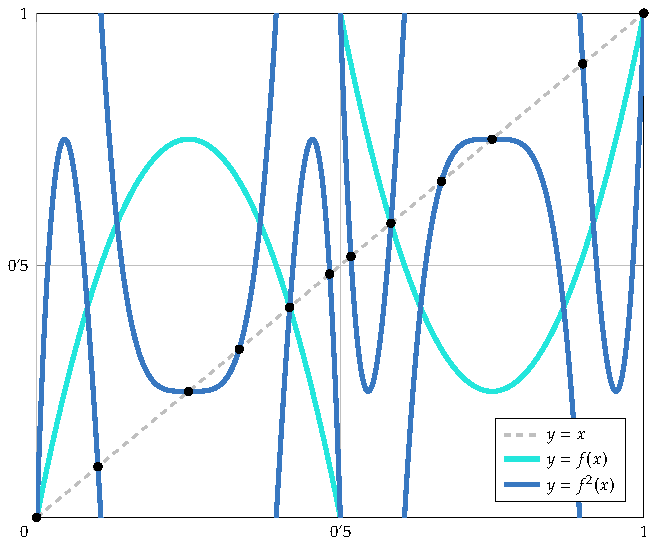
\includegraphics{./plot1/main.pdf}
    \end{figure}
    Como $f$ tiene 4 puntos fijos y $f^2$ tiene 12 puntos fijos, se concluye que hay $\frac{12-4}{2} = 4$ órbitas $2$-periódicas.
\end{solution}

\begin{exercise}
    Se considera el sistema dinámico discreto $(S)$ en el que $I = [0,1]$ y
    \[f(x) = \begin{cases}
        \frac{3}{2}x & $ si $ 0 \leq x < \frac{1}{2}, \\
        \frac{3}{2}(1-x) & $ si $ \frac{1}{2} \leq x \leq 1.
    \end{cases}\]
    Dibujar las gráficas de $f$, $f^2$ y $f^3$. Deducir qué numero de órbitas estacionarias y periódicas de periodo $2$ y $3$ hay, así como su estabilidad.
\end{exercise}

\begin{solution}
    Las órbitas estacionarias son las formadas por puntos fijos de $f$. Si $0 \leq x < \frac{1}{2}$, se tiene
    \[f(x) = x \iff \frac{3}{2}x = x \iff x = 0,\]
    mientras que si $\frac{1}{2} \leq x \leq 1$, se cumple
    \[f(x) = x \iff \frac{3}{2}(1-x) = x \iff \frac{5}{2}x = \frac{3}{2} \iff x = \frac{3}{5} = 0'6.\]
    Por tanto, las órbitas estacionarias del sistema son $\{l_1\}$ y $\{l_2\}$, donde $l_1 = 0$ y $l_2 = 0'6$. Además, $f$ es clase $1$ en $[0,\frac{1}{2}) \cup (\frac{1}{2},1]$ y
    \[f'(x) = \begin{cases}
        \frac{3}{2} & $ si $ 0 \leq x < \frac{1}{2}, \\
        -\frac{3}{2} & $ si $ \frac{1}{2} < x \leq 1.
    \end{cases}\]
    Como $|f'(l_1)| = |f'(l_2)| = \frac{3}{2} > 1$, las dos órbitas estacionarias del sistema son inestables.

    Por otra parte, para estudiar si hay órbitas $2$-periódicas y $3$-periódicas, se halla el número de puntos fijos de $f$, $f^2$ y $f^3$.
    \begin{figure}[H]
        \centering
        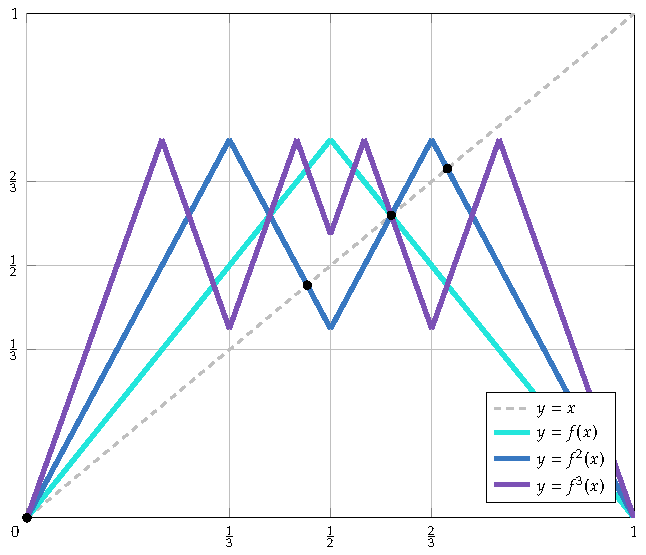
\includegraphics{./plot2/main.pdf}
    \end{figure}
    Se observa que $f$ tiene $2$ puntos fijos, $f^2$ tiene $4$ puntos fijos y $f^3$ tiene $2$ puntos fijos. Utilizando la fórmula
    \[\textup{n.º de órbitas } p \textup{-periódicas} = \frac{1}{p}\Bigl(\textup{n.º de ptos. fijos de } f^p - \sum_{j \mid p, \ j \neq p} j \cdot \textup{n.º de órbitas } j \textup{-periódicas}\Bigr),\]
    se obtiene que el número de órbitas $2$-periódicas es $\frac{1}{2}(4-2) = 1$, y el número de órbitas $3$-periódicas es $\frac{1}{3}(2-2) = 0$.

    La única órbita $2$-periódica es $\{p_1,p_2\}$, siendo $p_1$ y $p_2$ puntos fijos de $f^2$ que no son puntos fijos de $f$. Se tiene que
    \[f^2(x) = \begin{cases}
        \frac{9}{4}x & $ si $ 0 \leq x < \frac{1}{3}, \\
        \frac{3}{2}(1-\frac{3}{2}x) & $ si $ \frac{1}{3} \leq x < \frac{1}{2}, \\
        \frac{3}{2}(1-\frac{3}{2}(1-x)) & $ si $ \frac{1}{2} \leq x < \frac{2}{3}, \\
        \frac{9}{4}(1-x) & $ si $ \frac{2}{3} \leq x \leq 1. 
    \end{cases}\]
    En la gráfica se observa que $p_1 \in (\frac{1}{3},\frac{1}{2})$ y $p_2 \in (\frac{2}{3},1)$. Como
    \begin{align*}
        \frac{3}{2}\Bigl(1-\frac{3}{2}x\Bigr) = x \iff x+\frac{9}{4}x = \frac{3}{2} \iff x = \frac{3}{2}\cdot \frac{4}{13} = \frac{6}{13},
    \end{align*}
    entonces $p_1 = \frac{6}{13}$. Y como
    \begin{align*}
        \frac{9}{4}(1-x) = x \iff x+\frac{9}{4}x = \frac{9}{4} \iff x = \frac{9}{4} \cdot \frac{4}{13} = \frac{9}{13},
    \end{align*}
    entonces $p_2 = \frac{9}{13}$. Por otra parte,
    \[(f^2)'(x) = \begin{cases}
        \frac{9}{4} & $ si $ 0 \leq x < \frac{1}{3}, \\
        -\frac{9}{4} & $ si $ \frac{1}{3} < x < \frac{1}{2}, \\
        \frac{9}{4} & $ si $ \frac{1}{2} < x < \frac{2}{3}, \\
        -\frac{9}{4} & $ si $ \frac{2}{3} < x \leq 1.
    \end{cases}\]
    Como $|(f^2)'(p_1)| = |(f^2)'(p_2)| = \frac{9}{4} > 1$, la órbita $\{p_1,p_2\}$ es inestable.
\end{solution}

\begin{exercise}
    Se considera el sistema dinámico discreto $(S)$.
    \begin{enumerate}
        \item Si la función $f$ es continua, demostrar que entre los dos estados de una órbita $2$-periódica hay necesariamente un equilibrio $l$.
        \item Mostrar, con un ejemplo, que este resultado no es cierto si $f$ no es continua.
    \end{enumerate}
\end{exercise}

\begin{solution}
    \hfill
    \begin{enumerate}
        \item Sea $\{p_1,p_2\}$ una órbita $2$-periódica. Supóngase, sin pérdida de generalidad, que $p_1 < p_2$. Sea $g \colon [p_1,p_2] \to \R$ la función dada por $g(x) = f(x)-x$. Como $f$ es continua, $g$ también lo es. Además, $g(p_1) = f(p_1)-p_1 = p_2-p_1$ y $g(p_2) = f(p_2)-p_2 = p_1-p_2$, luego $g(p_1)$ y $g(p_2)$ tienen distinto signo. Por el teorema de Bolzano, existe $l \in (p_1,p_2)$ tal que $g(l) = 0$, es decir, $f(l) = l$.
        \item Considérese la función $f \colon [-1,1] \to \R$ dada por
        \[f(x) = \begin{cases}
            1 & $ si $ 0 \leq x < \frac{1}{2}, \\
            0 & $ si $ \frac{1}{2} \leq x \leq 1.
        \end{cases}\]
        Se tiene que
        \[f^2(x) = \begin{cases}
            1 & $ si $ 0 \leq f(x) < \frac{1}{2}, \\
            0 & $ si $ \frac{1}{2} \leq f(x) \leq 1.
        \end{cases} = \begin{cases}
            0 & $ si $ 0 \leq x < \frac{1}{2}, \\
            1 & $ si $ \frac{1}{2} \leq x \leq 1.
        \end{cases}\]
        Como $f$ no tiene puntos fijos y $f^2$ tiene dos puntos fijos, $0$ y $1$, se concluye que solo hay una órbita $2$-periódica y entre sus estados no hay ningún punto fijo de $f$.
    \end{enumerate}
\end{solution}

\begin{exercise}
    Dado $c = -1+i$, determinar las órbitas estacionarias y $2$-periódicas del sistema dinámico complejo
    \[z_{n+1} = z_n^2 + c.\]
\end{exercise}

\begin{solution}
    Sea $f \colon \C \to \C$ la función dada por $f(z) = z^2+c$. Se trata de hallar los puntos fijos de $f$ y $f^2$. Por un lado,
    \[f(z) = z \iff z^2+c = z \iff z^2-z+c = 0 \iff z = \frac{1\pm \sqrt{1-4c}}{2} = \frac{1\pm \sqrt{5-4i}}{2}\]
    Los puntos fijos de $f$ son $l_1 = \frac{1+ \sqrt{5-4i}}{2}$ y $l_2 = \frac{1- \sqrt{5-4i}}{2}$, así que las órbitas estacionarias son $\{l_1\}$ y $\{l_2\}$. Para hallar las órbitas $2$-periódicas, se estudian los puntos fijos de $f^2$. Se tiene que
    \begin{align*}
        f^2(z) = z &\iff  (z^2+c)^2+c = z \iff z^4+2cz^2-z+c^2+c = 0 \\
        &\iff z^4+(-2+2i)z^2-z-2i-1+i = 0 \iff z^4+(-2+2i)z^2-z-(1+i) = 0.
    \end{align*}
    Esta ecuación tiene cuatro soluciones distintas, así que $f^2$ tiene $4$ puntos fijos y por tanto el número de órbitas $2$-periódicas es $\frac{1}{2}(4-2) = 1$. Esta órbita está formada por puntos fijos de $f^2$ que no son puntos fijos de $f$, lo que permite afirmar que los puntos fijos de $f$ son raíces del polinomio $z^4+(-2+2i)z^2-z-(1+i) = 0$. En consecuencia, este polinomio es divisible entre $(z-l_1)(z-l_2)$. Una sarta de cuentas que no merece la pena reproducir demuestra que
    \[z^4+(-2+2i)z^2-z-(1+i) = (z^2+z+i)(z-l_1)(z-l_2)\]
    Como
    \[z^2+z+i = 0 \iff \frac{-1\pm\sqrt{1-4i}}{2},\]
    se concluye que la única órbita $2$-periódica es $\{p_1,p_2\}$, donde $p_1 = \frac{-1+\sqrt{1-4i}}{2}$ y $p_1 = \frac{-1-\sqrt{1-4i}}{2}$.
\end{solution}

\begin{exercise}
    Se considera el sistema dinámico $(S)$ con $I = \R$ y
    \[f_\mu (x) = x^2+\mu.\]
    \begin{enumerate}
        \item Estudiar las órbitas estacionarias y $2$-periódicas, así como su estabilidad, en los casos $\mu = 1$, $\mu = \frac{1}{8}$, $\mu = -\frac{1}{2}$ y $\mu = -1$. Deducir, en cada uno de los casos, la mayor información posible sobre el comportamiento asintótico de las órbitas.
        \item Discutir qué tipo de bifurcación ocurre cuando $\mu$ pasa por los valores $-\frac{3}{4}$ y $\frac{1}{4}$.
        \item Con ayuda del diagrama de órbitas, estudiar qué otros tipos de bifurcaciones aparecen cuando varía el parámetro.
    \end{enumerate}
\end{exercise}

\begin{solution}
    \hfill
    \begin{enumerate}
        \item Se hallan los puntos fijos de $f$ y $f^2$. Se tiene
        \[f_\mu(x) = x \iff x^2-x+\mu = 0 \iff x = \frac{1 \pm \sqrt{1-4\mu}}{2},\]
        mientras que 
        \begin{align*}
            f_\mu^2(x) = x &\iff (x^2+\mu)^2+\mu = x \iff x^4+2\mu x^2-x+\mu^2+\mu = 0.
        \end{align*}
        Por otro lado, $|f_\mu'(x)| = 2|x|$ para todo $x \in \R$.
        \begin{itemize}
            \item Para $\mu = 1$, $f_\mu$ no tiene puntos fijos y por tanto no hay órbitas estacionarias. Además, puede comprobarse que el polinomio $x^4+2x^2-x+2$ no tiene raíces reales, así que $f_\mu^2$ no tiene puntos fijos y por tanto tampoco hay órbitas $2$-periódicas.
            \item Para $\mu = \frac{1}{8}$, los puntos fijos de $f_\mu$ son
            \[l_1 = \frac{1+\sqrt{\frac{1}{2}}}{2} = \frac{\sqrt{2}+1}{2\sqrt{2}} \approx 0'85355339059, \qquad l_2 = \frac{1-\sqrt{\frac{1}{2}}}{2} = \frac{\sqrt{2}-1}{2\sqrt{2}} \approx 0'1464466094.\]
            Por tanto, las órbitas estacionarias son $\{l_1\}$ y $\{l_2\}$. Como $|f_\mu'(l_1)| = 2l_1 > 1$ y $|f_\mu'(l_2)| = 2l_2 < 1$, la primera órbita es inestable y repulsora, mientras que la segunda es asintóticamente estable. Por otra parte, se prueba que las raíces reales del polinomio $x^4+\frac{1}{4}x^2-x+\frac{9}{64}$ son $l_1$ y $l_2$, así que no hay órbitas $2$-periódicas.
            \item Para $\mu = -\frac{1}{2}$, los puntos fijos de $f_\mu$ son
            \[l_1 = \frac{1+\sqrt{3}}{2} \approx 1'36602540378, \qquad l_2 = \frac{1-\sqrt{3}}{2} \approx -0'36602540378 \]
            En consecuencia, las órbitas estacionarias son $\{l_1\}$ y $\{l_2\}$. Como $|f_\mu'(l_1)| = 2l_1 > 1$ y $|f_\mu'(l_2)| = -2l_2 < 1$, la primera órbita es asintóticamente estable, mientras que la segunda es inestable y repulsora. Por otra parte, se prueba que las raíces reales del polinomio $x^4-x^2-x-\frac{1}{4}$ son $l_1$ y $l_2$, así que no hay órbitas $2$-periódicas.
            \item Para $\mu = -1$, los puntos fijos de $f_\mu$ son
            \[l_1 = \frac{1+\sqrt{5}}{2} \approx 1'61803398875, \qquad l_2 = \frac{1-\sqrt{5}}{2} \approx -0'61803398875 \]
            En consecuencia, las órbitas estacionarias son $\{l_1\}$ y $\{l_2\}$. Como $|f_\mu'(l_1)| = 2l_1 > 1$ y $|f_\mu'(l_2)| = -2l_2 > 1$, ambas órbitas son inestables y repulsoras. Por otra parte, se prueba que las raíces reales del polinomio $x^4-2x^2-x$ son $l_1$, $l_2$, $p_1 = 0$ y $p_2 = -1$, así que la única órbita $2$-periódica es $\{p_1,p_2\}$. Se tiene que $|(f_\mu^2)'(x)| = 4|x|(x^2+\mu)$, luego $|(f_\mu^2)'(p_1)| = 0 < 1$ y por tanto $p_1$ es un equilibrio asintóticamente estable para $f^2$, obteniéndose que la órbita $\{p_1,p_2\}$ es asintóticamente estable.
        \end{itemize}
        \item Se observa que para $\mu > \frac{1}{4}$ no hay puntos de equilibrio, pues $1-4\mu < 0$ y por tanto la ecuación $f_\mu(x) = x$ no tiene soluciones reales. Para $-\frac{3}{4} < \mu \leq \frac{1}{4}$, hay un equilibrio estable y no hay órbitas $2$-periódicas, mientras que $\mu < -\frac{3}{4}$, aparece una órbita $2$-periódica asintóticamente estable que acaba siendo inestable.
        \begin{figure}[H]
        \centering
        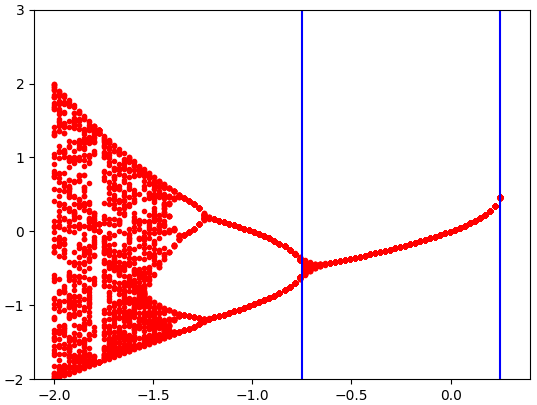
\includegraphics[scale = 0.8]{./img/Figure_1.png}
        \end{figure}
        \item En el diagrama de bifurcación también se observa que alrededor de $\mu = 1'25$, la órbita $2$-periódica se vuelve inestable y aparece una órbita $4$-periódica asintóticamente estable, mientras que alrededor de $\mu = 1'40$, la órbita $4$-periódica se torna inestable. Para $\mu < -1'40$, aparecen órbitas de mayor periodo y el sistema entra en un régimen caótico.
        \begin{figure}[H]
        \centering
        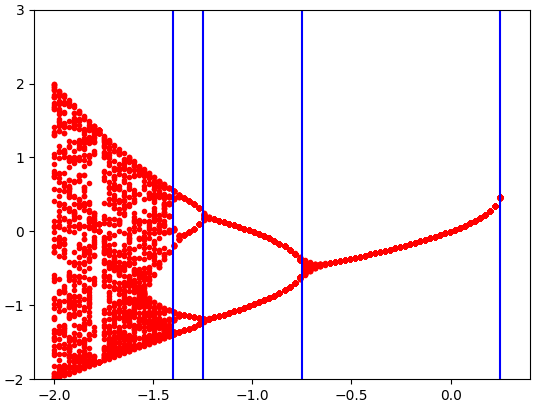
\includegraphics[scale = 0.8]{./img/Figure_2.png}
        \end{figure}
    \end{enumerate}
\end{solution}

\begin{exercise}
    Se considera el sistema dinámico $(S)$ con $I = \R$ y
    \[f_\mu (x) = x^3-\mu x.\]
    \begin{enumerate}
        \item Estudiar las órbitas estacionarias y $2$-periódicas, así como su estabilidad, para los valores $\mu = -2$, $\mu = 0$, $\mu = 1$ y $\mu = \frac{3}{2}$. Deducir, en cada uno de los casos, la mayor información posible sobre el comportamiento asintótico de las órbitas.
        \item Discutir qué tipo de bifurcación ocurre cuando $\mu$ pasa por los valores $-1$ y $1$.
        \item Con ayuda del diagrama de órbitas, estudiar qué otros tipos de bifurcaciones aparecen cuando varía el parámetro.
    \end{enumerate}
\end{exercise}

\begin{solution}
    \hfill
    \begin{enumerate}
        \item Se hallan los puntos fijos de $f$ y $f^2$. Se tiene que
        \[f_\mu(x) = x \iff x^3-(\mu+1)x = 0 \iff x(x^2-(\mu+1)) = 0.\]
        Por tanto, $l_1 = 0$ siempre es un punto fijo de $f_\mu$, y si $\mu \geq -1$, entonces $l_2 = \sqrt{\mu+1}$ y $l_3 = -\sqrt{\mu+1}$ también son puntos fijos de $f_\mu$ Además, 
        \begin{align*}
            f_\mu^2(x) = x &\iff (x^3-\mu x)^3-\mu(x^3-\mu x) = x \iff x^3(x^2-\mu)^3 -\mu x^3 + (\mu^2-1)x = 0 \\
            &\iff x = 0 \textup{ ó } x^2(x^2-\mu)^3 - \mu x^2 + \mu^2 - 1 = 0.
        \end{align*}
        Por otro lado, $|f_\mu'(x)| = |3x^2-\mu|$ para todo $x \in \R$.
        \begin{itemize}
            \item Para $\mu = -2$, $l_1 = 0$ es el único punto fijo de $f_\mu$, y es inestable y repulsor porque $|f_\mu'(l_1)| = |\mu| = 2 > 1$. Además, puede comprobarse que el polinomio $x^2(x^2+2)^3+2x^2+3$ no tiene raíces reales, así que $f_\mu^2$ no tiene puntos fijos y por tanto no hay órbitas $2$-periódicas.
            \item Para $\mu = 0$, los puntos fijos de $f_\mu$ son
            \[l_1 = 0, \qquad l_2 = \sqrt{\mu+1} = 1, \qquad l_3 = -\sqrt{\mu+1} = -1.\]
            Por tanto, las órbitas estacionarias son $\{l_1\}$, $\{l_2\}$ y $\{l_3\}$. Como $|f_\mu'(l_1)| = 0 < 1$, $|f_\mu'(l_2)| = 3 > 1$ y $|f_\mu'(l_3)| = 3 > 1$, la primera órbita es asintóticamente estable, mientras que las dos últimas son inestables y repulsoras. Por otra parte, se prueba que las raíces reales del polinomio $x^8-1$ son $l_2$ y $l_3$, que también son puntos fijos de $f$. Por tanto, tampoco hay órbitas $2$-periódicas.
            \item Para $\mu = 1$, los puntos fijos de $f_\mu$ son
            \[l_1 = 0, \qquad l_2 = \sqrt{\mu+1} = \sqrt{2}, \qquad l_3 = -\sqrt{\mu+1} = -\sqrt{2}.\]
            En consecuencia, las órbitas estacionarias son $\{l_1\}$, $\{l_2\}$ y $\{l_3\}$. Como $|f_\mu'(l_1)| = 0 < 1$, $|f_\mu'(l_2)| = 5 > 1$ y $|f_\mu'(l_3)| = 5 > 1$, la primera órbita es asintóticamente estable, mientras que las dos últimas son inestables y repulsoras. Por otra parte, se prueba que las raíces reales del polinomio $x^2(x^2-1)^3-x^2$ son $l_1$, $l_2$ y $l_3$, que también son puntos fijos de $f$. Por tanto, tampoco hay órbitas $2$-periódicas.
            \item Para $\mu = \frac{3}{2}$, los puntos fijos de $f_\mu$ son
            \[l_1 = 0, \qquad l_2 = \sqrt{\mu+1} = \frac{\sqrt{5}}{\sqrt{2}} = \frac{\sqrt{10}}{2}, \qquad l_3 = -\sqrt{\mu+1} = -\frac{\sqrt{10}}{2}.\]
            En consecuencia, las órbitas estacionarias son $\{l_1\}$, $\{l_2\}$ y $\{l_3\}$. Como $|f_\mu'(l_1)| = 0 < 1$, $|f_\mu'(l_2)| = |3\frac{10}{4}-\frac{3}{2}| = 6 > 1$ y $|f_\mu'(l_3)| = 6 > 1$, la primera órbita es asintóticamente estable, mientras que las dos últimas son inestables y repulsoras. Por otra parte, se prueba que las raíces reales del polinomio $x^2(x^2-\frac{3}{2})^3-\frac{3}{2}x^2+\frac{5}{4}$ son $l_2$, $l_3$, $p_1 = \frac{\sqrt{2}}{2}$ y $p_2 = -\frac{\sqrt{2}}{2}$. Por tanto, la única órbita $2$-periódica es $\{p_1,p_2\}$. Se tiene que
            \[|(f_\mu^2)'(x)| = 3(3x^2-\mu)(x^3-\mu x)^2-\mu(3x^2-\mu) = (3x^2-\mu)(3(x^3-\mu x)^2 - \mu).\]
            Como $3p_1^2-\frac{3}{2} = 0$, entonces $|(f_\mu^2)'(p_1)| = 0 < 1$ y se concluye que la órbita $\{p_1,p_2\}$ es asintóticamente estable.
        \end{itemize}
        \item Se observa que para $\mu < -1$ no hay puntos de equilibrio, pues $\mu+1 < 0$ y por tanto la ecuación $f_\mu(x) = x$ no tiene soluciones reales. Para $-1 < \mu < 1$, no hay órbitas periódicas de periodo mayor que $1$, mientras que para $\mu > 1$, aparece una órbita $2$-periódica que se acaba volviendo inestable.
        \begin{figure}[H]
        \centering
        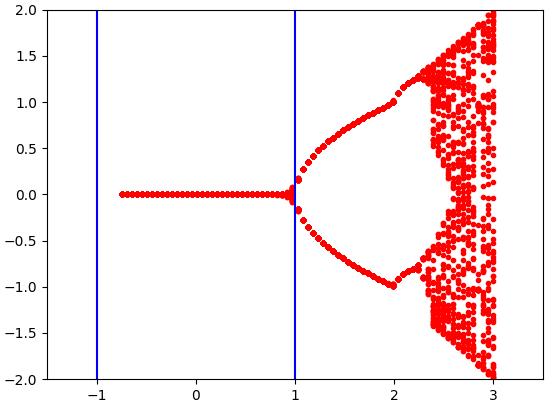
\includegraphics[scale = 0.8]{./img/Figure_3.png}
        \end{figure}
        \item En el diagrama de bifurcación también se observa que para $-0'75 \leq \mu \leq 1$, hay un equilibrio estable, mientras que alrededor de $\mu = 2.3$, la órbita $2$-periódica se torna inestable. Para $\mu > 2.3$, aparecen órbitas de mayor periodo y el sistema entra en un régimen caótico.
        \begin{figure}[H]
        \centering
        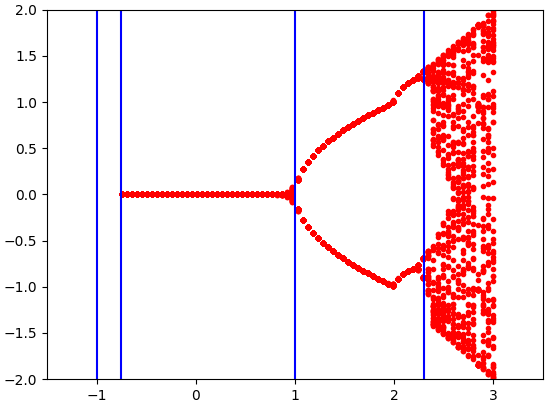
\includegraphics[scale = 0.8]{./img/Figure_4.png}
        \end{figure}
    \end{enumerate}
\end{solution}

\begin{exercise}
    Se considera el sistema dinámico $(S)$ con $I = \R$ y
    \[f_\mu (x) = \mu \sen(x).\]
    \begin{enumerate}
        \item Estudiar las órbitas estacionarias y $2$-periódicas, así como su estabilidad, para los valores $\mu = \frac{1}{2}$, $\mu = \frac{3}{2}$ y $\mu = \frac{5}{2}$. Deducir, en cada uno de los casos, la mayor información posible sobre el comportamiento asintótico de las órbitas.
        \item Discutir qué tipo de bifurcación ocurre cuando $\mu$ pasa por los valores $\mu = 1$ y $\mu \approx 2'26$.
        \item Con ayuda del diagrama de órbitas, estudiar qué otros tipos de bifurcaciones aparecen cuando varía el parámetro.
    \end{enumerate}
\end{exercise}

\begin{solution}
    Extremadamente similar a los ejercicios anteriores.
\end{solution}

\begin{exercise}
    Se considera el sistema dinámico $(S)$ con $I = \R$ y
    \[f_\mu (x) = \mu e^x.\]
    \begin{enumerate}
        \item Estudiar las órbitas estacionarias y $2$-periódicas, así como su estabilidad, para los valores $\mu = -3$, $\mu = -e^{-1}$, $\mu = e^{-1}$ y $\mu = 1$. Deducir, en cada uno de los casos, la mayor información posible sobre el comportamiento asintótico de las órbitas.
        \item Discutir qué tipo de bifurcación ocurre cuando $\mu$ pasa por los valores $-e$, $0$ y $e^{-1}$.
        \item Con ayuda del diagrama de órbitas, estudiar qué otros tipos de bifurcaciones aparecen cuando varía el parámetro.
    \end{enumerate}
\end{exercise}

\begin{solution}
    Extremadamente similar a los ejercicios anteriores.
\end{solution}

\begin{exercise}
    Se considera el sistema dinámico $(S)$ con $I = \R$ y
    \[f_\mu (x) = x+x^2+\mu.\]
    \begin{enumerate}
        \item Estudiar las órbitas estacionarias y $2$-periódicas, así como su estabilidad, para los valores $\mu = -1'2$, $\mu = -0'5$ y $\mu = 0'5$. Deducir, en cada uno de los casos, la mayor información posible sobre el comportamiento asintótico de las órbitas.
        \item Discutir qué tipo de bifurcación ocurre cuando $\mu$ pasa por los valores $-1$ y $0$.
        \item Con ayuda del diagrama de órbitas, estudiar qué otros tipos de bifurcaciones aparecen cuando varía el parámetro.
    \end{enumerate}
\end{exercise}

\begin{solution}
    Extremadamente similar a los ejercicios anteriores.
\end{solution}

\begin{exercise}
    Se considera el sistema dinámico $(S)$ con $I = \R$ y
    \[f_\mu(x) = x+\mu x^2.\]
    Estudiar sus equilibrios y sus dominios de atracción y repulsión.
\end{exercise}

\begin{solution}
    Se tiene que
    \[f_\mu(x) = x \iff \mu x^2 = 0 \iff x = 0 \textup{ ó } \mu = 0.\]
    Se barajan los siguientes casos:
    \begin{enumerate}
        \item Si $\mu = 0$, todos los números reales son equilibrios del sistema dinámico. Sea $l \in \R$. Se trata de estudiar el dominio de atracción y repulsión de $l$. Para todo $x \in \R$, usando que $x$ es punto fijo de $f$, se tiene
        \[\lim_{n\to\infty} f^n(x) = l \iff \lim_{n\to\infty} x = l \iff \iff x = l.\]
        De forma análoga,
        \[\lim_{n\to-\infty} f^n(x) = l \iff x = l.\]
        Por tanto, $S_l = \{l\}$ y $U_l = \{l\}$.
        \item Si $\mu \neq 0$, el único equilibrio del sistema dinámico es $l = 0$. Como $|f_\mu'(l)| = |1+2\mu l| = 1$, este equilibrio es no hiperbólico, así que se va a recurrir a razonamientos geométricos para determinar los dominios de atracción y de repulsión de $l$.
        \begin{itemize}
            \item Supóngase que $\mu > 0$. Entonces
            \[f_\mu'(x) > 0 \iff 2\mu x > -1 \iff x > -\frac{1}{2\mu},\]
            mientras que 
            \[f_\mu'(x) < 0 \iff 2\mu x < -1 \iff x < -\frac{1}{2\mu}.\]
            Así, $f_\mu$ es estricamente creciente en $(-\frac{1}{2\mu},\infty)$ y estrictamente decreciente en $(-\infty,-\frac{1}{2\mu})$. Los puntos de corte de la gráfica de $f$ con los ejes son $(0, 0)$ y $(-\frac{1}{\mu},0)$. Con esta información se puede esbozar la gráfica de $f$.
            \begin{figure}[H]
            \centering
            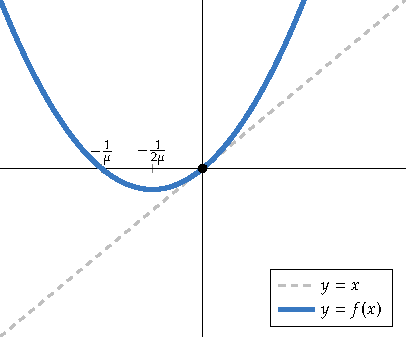
\includegraphics{./plot3/main.pdf}
            \end{figure}
            Dado $x_0 \in \R$, se observa que la sucesión definida por $x_{n+1} = f(x_n)$ se aleja de $ 0$ cuando $x_0 > 0$ y $x_0 < -\frac{1}{\mu}$, y se acerca a $0$ cuando $-\frac{1}{\mu} \leq x_0 \leq 0$. Por tanto, $S_0 = [-\frac{1}{\mu},0]$ y $U_0 = (-\infty,-\frac{1}{\mu})\cup [0,\infty)$.
            \item Supóngase que $\mu < 0$. Entonces
            \[f_\mu'(x) > 0 \iff 2\mu x > -1 \iff x < -\frac{1}{2\mu},\]
            mientras que 
            \[f_\mu'(x) < 0 \iff 2\mu x < -1 \iff x > -\frac{1}{2\mu}.\]
            Así, $f_\mu$ es estricamente decreciente en $(-\frac{1}{2\mu},\infty)$ y estrictamente creciente en $(-\infty,-\frac{1}{2\mu})$. Igual que antes, los puntos de corte de la gráfica de $f$ con los ejes son $(0, 0)$ y $(-\frac{1}{\mu},0)$. Con esta información se puede esbozar la gráfica de $f$.
            \begin{figure}[H]
            \centering
            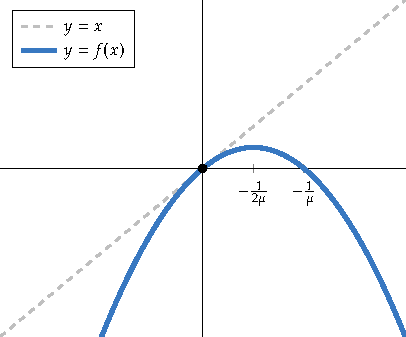
\includegraphics{./plot4/main.pdf}
            \end{figure}
            Dado $x_0 \in \R$, se observa que la sucesión definida por $x_{n+1} = f(x_n)$ se aleja de $ 0$ cuando $x_0 < 0$ y $x_0 > -\frac{1}{\mu}$, y se acerca a $0$ cuando $0 \leq x_0 \leq -\frac{1}{\mu}$. Por tanto, $S_0 = [0,-\frac{1}{\mu}]$ y $U_0 = (-\infty,0]\cup (-\frac{1}{\mu},\infty)$.
        \end{itemize}
    \end{enumerate}
\end{solution}

\begin{exercise}
    La población de insectos en un manglar sigue el modelo $(S)$ con $I = [0,\infty)$ y
    \[f(x) = \begin{cases}
        0'01x^2 & $ si $ 0 \leq x \leq K, \\
        0'01K^2e^{-r(x-K)} & $ en otro caso$,
    \end{cases}\]
    siendo $K = 1000$ y $r = 1'75 \cdot 10^{-4}$.
    \begin{enumerate}
        \item Probar que, con un cambio de variables adecuado, el modelo puede escribirse en la forma adimensional
        \[u_{n+1} = g(u_n), \qquad n = 0,1,2,\mathellipsis,\]
        siendo
        \[g(u) = \begin{cases}
            \alpha u^2 & $ si $ 0 \leq u \leq 1, \\
            \alpha e^{-\beta(u-1)} & $ en otro caso$,
        \end{cases}\]
        con $\alpha$ y $\beta$ dos constantes positivas a determinar. En los siguientes apartados se considerará la forma adimensional del modelo.
        \item Estudiar los equilibrios y su estabilidad.
        \item Estudiar el comportamiento asintótico del número de individuos en función del número inicial.
    \end{enumerate}
\end{exercise}

\begin{solution}
    En primer lugar, se observa que $f$ es continua en $I$ y que $f(I) \subset I$, así que el sistema dinámico considerado tiene sentido.
    \begin{enumerate}
        \item Nótese que $x$ y $K$ tienen las mismas unidades porque en la definición de $f$ aparece $x-K$. En consecuencia, el cambio de variables
        \[u = \frac{x}{K}\]
        es adimensional. Si $n = 0,1,2,\mathellipsis$, se tiene que
        \begin{align*}
            u_{n+1} = \frac{x_{n+1}}{K} = \frac{f(x_n)}{K} &= \begin{cases}
                \frac{0'01 x_n^2}{K} & $ si $ 0 \leq x \leq K, \\
                0'01Ke^{-r(x_n-K)} & $ en otro caso$.
            \end{cases} \\ &=  \begin{cases}
                \frac{0'01 u_n^2K^2}{K} & $ si $ 0 \leq uK \leq K, \\
                0'01Ke^{-r(u_nK-K)} & $ en otro caso$.
            \end{cases} \\ &= \begin{cases}
                0'01Ku_n^2 & $ si $ 0 \leq u \leq 1, \\
                0'01Ke^{-rK(u_n-1)} & $ en otro caso$.
            \end{cases}
        \end{align*}
        Sea $\alpha = 0'01K = 10$, sea $\beta = rK = 0'175$ y sea $g \colon I \to I$ la función dada por
        \[g(u) = \begin{cases}
            \alpha u^2 & $ si $ 0 \leq u \leq 1, \\
            \alpha e^{-\beta(u-1)} & $ en otro caso$.
        \end{cases} = \begin{cases}
            10 u^2 & $ si $ 0 \leq u \leq 1, \\
            10 e^{-0'175(u-1)} & $ en otro caso$.
        \end{cases}\]
        Los razonamientos anteriores prueban que el modelo se puede escribir como
        \[u_{n+1} = g(u_n), \qquad n = 0,1,2,\mathellipsis\]
        \item Si $0 \leq u \leq 1$, se tiene
        \[g(u) = u \iff \alpha u^2 = u \iff u = 0 \textup{ ó } u = \frac{1}{\alpha} = 0'1,\]
        mientras que si $u > 1$,
        \begin{align*}
            g(u) = u &\iff 10e^{-0'175(u-1)} = u.
        \end{align*}
        Puede probarse que esta ecuación tiene una única solución, $u \approx 4'98174$. Por otro lado,
        \[g'(u) = \begin{cases}
            20u & $ si $ 0 \leq u < 1, \\
            -1'75e^{-0'175(u-1)} & $ si $ u > 1.
        \end{cases}\]
        Los equilibrios del sistema son $l_1 = 0$, $l_2 = 0'1$ y $l_3 \approx 4'98174$. Se tiene que $|g'(l_1)| = 0 < 1$, $|g'(l_2)| = 20\cdot 0'1 = 2 > 1$ y $|g'(l_3)| = 1'75e^{-0'175(l_3-1)}| = 1'75\frac{l_3}{10} = 0'175l_3 \approx 0'8718045 < 1$. Por tanto, $l_1$ y $l_3$ son asintóticamente estables, meintras que $l_2$ es inestable y repulsor.
        \item Sea $u_0 \in [0,\infty)$ el número inicial de individuos. Se trata de estudiar geométricamente el comportamiento de la sucesión definida por $u_{n+1} = g(u_n)$, $n = 0,1,2,\mathellipsis$
        \begin{figure}[H]
            \centering
            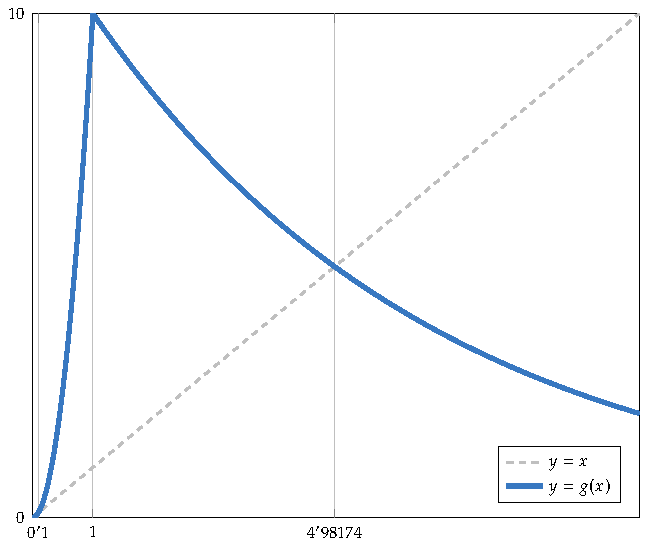
\includegraphics{./plot5/main.pdf}
        \end{figure}
        Se observa que:
        \begin{itemize}
            \item Si $0 \leq u_0 < 0'1$, entonces $\lim_{n\to\infty} u_n = 0$.
            \item Si $u_0 = 0'1$, entonces $\lim_{n\to\infty} u_n = 0'1$.
            \item Si $0'1 < u \leq l_3$, entonces $\lim_{n\to\infty} u_n = l_3$.
            \item Si $u > l_3$, entonces $\lim_{n\to\infty} u_n = l_3$.
        \end{itemize}
    \end{enumerate}
\end{solution}

\begin{exercise}
    La población de una especie sigue el modelo
    \[\begin{cases}
        x_0 \in [0,\infty), \\
        x_{n+1} = ax_ne^{-x_n}, \qquad n \geq 0,
    \end{cases}\]
    donde $a$ es un número real mayor que $0$.
    \begin{enumerate}
        \item Determinar los equilibrios y estudiar su estabilidad. ¿Para qué valores de $a$ se extingue la población, sea cual sea la condición inicial?
        \item Estudiar la existencia de órbitas $2$-periódicas para $a = 4$ y $a = 10$. En caso de haber alguna, determinar su tipo de estabilidad. ¿Para qué valor de $a$ se produce la primera bifurcación por duplicación del periodo?
        \item Con ayuda de un diagrama de órbitas, estudiar qué otras bifurcaciones se producen cuando $a$ aumenta.
        \item Comentar cuál es la evolución esperada de la especie en función del valor de $a$.
    \end{enumerate}
\end{exercise}

\begin{solution}
    Sea $f \colon [0,\infty)\to\R$ la función dada por $f(x) = axe^{-x}$. Es claro que $f$ es continua y que $f([0,\infty)) \subset [0,\infty)$, así que el sistema dinámico considerado tiene sentido.
    \begin{enumerate}
        \item Se tiene que
        \[f(x) = x \iff axe^{-x} = x \iff \textup{x = 0} \textup{ ó } x = \log(a).\]
        Por otro lado, $f'(x) = ae^{-x}-axe^{-x} = ae^{-x}(1-x)$ para todo $x \geq 0$. Se distinguen dos casos:
        \begin{itemize}
            \item Si $ 0 < a < 1$, entonces $\log(a) < 0$ y por tanto el único equilibrio es $l = 0$. Como $|f'(l)| = a < 1$, dicho equilibrio es asintóticamente estable.
            \item Si $a \geq 1$, entonces $\log(a) \geq 0$ y por tanto los equilibrios son $l_1 = 0$ y $l_2 = \log(a)$. Además, $|f'(l_1)| = a$ y $|f'(l_2)| = |1-\log(a)|$. Se distinguen otros cuantos casos:
            \begin{itemize}
                \item Si $a = 1$, entonces $|f'(l_1)| = 1$ y $|f'(l_2)| = 0 <1 $, luego $l_1$ es un equilibrio no hiperbólico y $l_2$ es un equilibrio asintóticamente estable. Para estudiar la estabilidad de $l_1$, se observa que $f'(x) = ae^{-x}(1-x) > 0$ para todo $x \in (l_1,1)$, luego $f$ es estrictamente creciente en $(l_1,1)$. Como además $f(x) = xe^{-x} < x$ para todo $x \in (l_1,1)$, entonces $l_1$ es un equilibrio asintóticamente estable.
                \item Si $1 < a \leq e$, entonces $0 <\log(a) \leq 1$ y por tanto se tiene $|f'(l_1)| = a > 1$ y $|f'(l_2)| = |1-\log(a)| = 1-\log(a) < 1$. Así, $l_1$ es un equilibrio inestable y repulsor y $l_2$ es un equilibrio asintóticamente estable.
                \item Si $e < a < e^2$, entonces $1 <\log(a) < 2$ y por tanto se tiene $|f'(l_1)| = a > 1$ y $|f'(l_2)| = |1-\log(a)| = \log(a)-1 < 1$. Así, $l_1$ es un equilibrio inestable y repulsor y $l_2$ es un equilibrio asintóticamente estable.
                \item Si $a = e^2$, entonces $|f'(l_1)| = e^2 > 1$ y $|f'(l_2)| = |1-\log(e^2)| = 1$, luego $l_1$ es un equilibrio inestable y repulsor y $l_2 = \log(e^2) = 2$ es un equilibrio no hiperbólico.
                \begin{figure}[H]
                    \centering
                    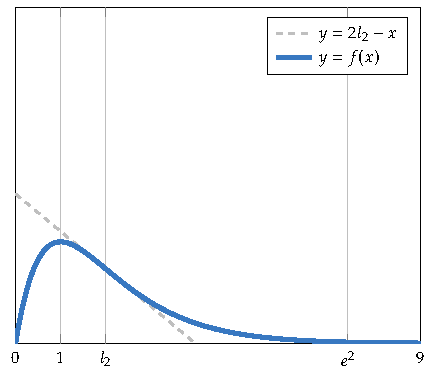
\includegraphics{./plot6/main.pdf}
                \end{figure}
                Se observa que existe $\varepsilon > 0$ tal que $f$ es decreciente en $(l_2-\varepsilon,l_2+\varepsilon)$, $f(x) < 2l_2-x$ para todo $x \in (l_2-\varepsilon,l_2)$, y $f(x) > 2l_2-x$ para todo $x \in (l_2,l_2+\varepsilon)$. En consecuencia, $l_2$ es un equilibrio asintóticamente estable.
                \item Si $a > e^2$, entonces se tiene $\log(a) > 2$ y, consecuentemente, $|f'(l_1)| = a > 1$ y $|f'(l_2)| = |1-\log(a)| = \log(a)-1 > 1$. Así, $l_1$ y $l_2$ son equilibrios inestables y repulsores.
            \end{itemize}
        \end{itemize}

        Si $0 < a < 1$, la población siempre se extingue independientemente de la población inicial, pues el único equilibrio es $l = 0$ y es estable y atractor. 
        \item Para estudiar las órbitas $2$-periódicas, se hallan los puntos fijos de $f^2$:
        \begin{align*}
            f^2(x) &= x \iff a(axe^{-x})e^{-(axe^{-x})} = x \iff a^2xe^{-x(1+ae^{-x})} = x
        \end{align*}
        Se observa que $l_1 = 0$ es un punto fijo de $f^2$. Para $x \neq 0$,
        \begin{align*}
            f^2(x) &= x \iff a^2e^{-x(1+ae^{-x})} = 1 \iff e^{-x(1+ae^{-x})} = a^{-2} \iff -x(1+ae^{-x}) = -2\log(a).
        \end{align*}

        Para $a = 4$, se prueba que la únuica solución de la ecuación anterior es $l_2 = \log(4)$, que es también punto de $f$. Por tanto, los dos puntos fijos de $f^2$ son también puntos fijos de $f$, así que no hay órbitas $2$-periódicas.
        
        Para $a = 10$, las soluciones de la ecuación son $l_2 = \log(10)$, $p_1 \approx 0'934596$ y $p_2 \approx 3'67057$. Como hay dos puntos fijos de $f^2$ que no son puntos fijos de $f$, la única órbita $2$-periódica es $\{p_1,p_2\}$. Se tiene que
        \[|f'(p_1)f'(p_2)| = |10e^{-p_1}(1-p_1)| \cdot |10e^{-p_2}(1-p_2)| \approx 0'174667 < 1,\]
        así que la órbita es asintóticamente estable.

        En el diagrama de bifurcación de $f$ se observa que en $a \approx 7'3$ se produce la primera bifurcación por duplicación del periodo, pues para $a<7'3$ no hay órbitas $2$-periódicas, mientras que para $a > 7'3$ sí las hay.
        \begin{figure}[H]
        \centering
        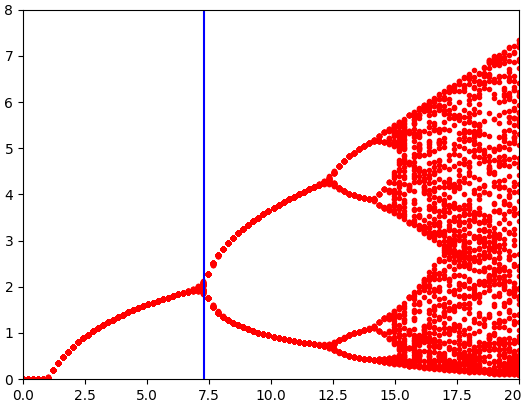
\includegraphics[scale = 0.8]{./img/Figure_5.png}
        \end{figure}
        \item También se observa en el diagrama de bifurcación que en $a = 1$ aparece un equilibrio asintóticamente estable no nulo. Enn $a \approx 12'2$, la órbita $2$-periódica se vuelve inestable y aparece una órbita $4$-periódica asintóticamente estable. En $a \approx 14'2$, la órbita $4$-periódica se vuelve inestable y aparece una órbita $8$-perióica asintóticamente estable. Finalmente, para $a > 14'2$ aparecen órbitas estables de cada vez mayor periodo y el sistema transiciona a un régimen caótico.
        \begin{figure}[H]
        \centering
        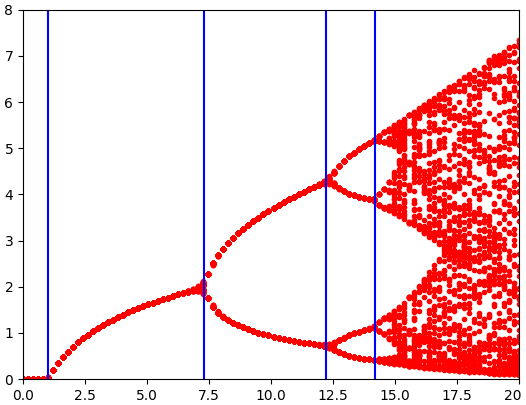
\includegraphics[scale = 0.8]{./img/Figure_6.png}
        \end{figure}
        \item Si $0 < a <1$, la especie siempre se extingue porque el único equilibrio es $l = 0$, y es asintóticamente estable. Si $1 \leq a < 7'3$, la especie tiende al equilibrio $l = \log(a)$, pues dicho equilibrio es asintóticamente estable. Para $7'3 \leq a < 12'2$, la especie sigue un patrón $2$-periódico. Para $a \leq 12'2 < 14'2$, la especie sigue un patrón $4$-periódico. Finalmente, para $a > 14'2$, la evolución de la población se vuelve impredecible.
    \end{enumerate}
\end{solution}

\begin{exercise}
    El sistema dinámico discreto
    \[t_{n+1} = \frac{K}{t_n-90}+100, \qquad n = 0,1,\mathellipsis\]
    modela el tiempo $t_n$ (medido en microsegundos) que tarda en llegar la señal eléctrica inducida por un marcapasos desde el atria (lugar que se estimula) hasta los ventrículos del corazón, en el $n$-ésimo latido; $K$ es una constante positiva.
    \begin{enumerate}
        \item Probar que, usando un cambio de variables adecuado, el modelo puede ser reescrito en la forma adimensional
        \[x_{n+1} = \frac{1}{x_n}+\alpha, \qquad n = 0,1,\mathellipsis\]
        siendo $\alpha > 0$ un parámetro. Sabiendo que $t_n$ es siempre mayor que $90$, ¿en qué intervalo toma valores la variable adimensional $x_n$?
        \item Estudiar los equilibrios y su estabilidad (solo se considerarán los que pertenezcan al intervalo determinado en el apartado anterior).
        \item Con ayuda del apartado anterior y de los diagramas web, describe el comportamiento esperado de $t_n$ cuando $n$ tiende a infinito.
        \item ¿Qué ocurre si $\alpha = 0$?
    \end{enumerate}
\end{exercise}

\begin{solution}
    \hfill
    \begin{enumerate}
        \item Llámese $T$ a la unidad para medir el tiempo (microsegundos, en este caso). Como $[t_n-90] = T$ y $[\frac{K}{t_n-90}] = [t_{n+1}-100]= T$, entonces $[K] = T^2$. Considérese el cambio de variales
        \[x = \frac{t-90}{\sqrt{K}},\]
        que es adimensional porque $[\sqrt{K}] = T$ y $[t-90] = T$. Se tiene que
        \begin{align*}
            x_{n+1} = \frac{t_{n+1}-90}{\sqrt{K}} =  \frac{\frac{K}{t_n-90}+10}{\sqrt{K}} = \frac{K}{(t_n-90)\sqrt{K}} + \frac{10}{\sqrt{K}} = \frac{\sqrt{K}}{t_n-90}+\frac{10}{\sqrt{K}} = \frac{1}{x_n}+\frac{10}{\sqrt{K}}.
        \end{align*}    
        Por tanto, el modelo se puede escribir en la forma
        \[x_{n+1} = \frac{1}{x_n}+\alpha, \qquad n = 0,1,\mathellipsis,\]
        siendo $\alpha = \frac{10}{\sqrt{K}} > 0$. Además,
        \[t_n > 90 \iff \sqrt{K}x_n+90 > 90 \iff \sqrt{K}x_n > 0 \iff x_n > 0,\]
        así que el intervalo en el que toma valores la nueva variable adimensional es $(0,\infty)$.
        \item Se considera la función $f \colon (0,\infty) \to \R$ dada por $f(x) = \frac{1}{x}+\alpha$. Nótese que $f$ es continua y verifica $f((0,\infty))\subset(0,\infty)$, así que el sistema dinámico a considerar tiene perfecto sentido. Por otro lado,
        \[f(x) = x \iff \frac{1}{x}+\alpha = x \iff x^2-\alpha x -1 = 0 \iff x = \frac{\alpha\pm \sqrt{\alpha^2+4}}{2}.\]
        Ahora bien,
        \[\frac{\alpha}{2}-\frac{\sqrt{\alpha^2+4}}{2} > 0 \iff \alpha>\sqrt{\alpha^2+4} \iff \alpha^2 > \alpha^2+4,\]
        y esto último es falso. Por tanto, el único equilibrio del sistema dinámico es $l = \frac{\alpha+\sqrt{\alpha^2+4}}{2}$. Como $f'(x) = -\frac{1}{x^2}$, entonces \[|f'(l_1)| = \frac{1}{l_1^2} = \frac{1}{\frac{\alpha^2}{4}+\frac{\alpha^2+4}{4}+\alpha\sqrt{\alpha^2+4}} = \frac{1}{\frac{\alpha^2}{2}+\alpha\sqrt{\alpha^2+4}+1} < 1,\]
        así que dicho equilibrio es asintóticamente estable.
        \item Tomando $\alpha = 1$ (es decir, $K = 100$) y representando los primeros términos de la sucesión $\{x_n\}_{n=0}^\infty$ para distintos valores de $x_0$, se observa que la sucesión converge a $l \approx 1'61803$ para cualquier $x_0 > 0$. Por tanto, la sucesión $\{t_n\}_{n=0}^\infty$ convergerá a $\sqrt{K}l+90 = 10l+90 \approx 106'18034$ para cualquier $t_0 > 90$.
        \begin{figure}[H]
            \centering
            \begin{subfigure}[b]{0.49\textwidth}
            \centering
            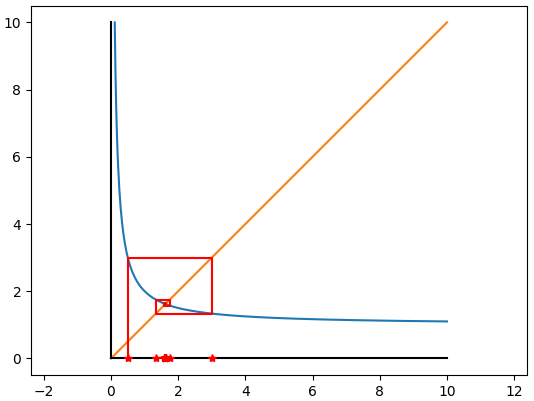
\includegraphics[scale = 0.5]{./img/Figure_7.png}
            \end{subfigure}
            \begin{subfigure}[b]{0.49\textwidth}
            \centering
            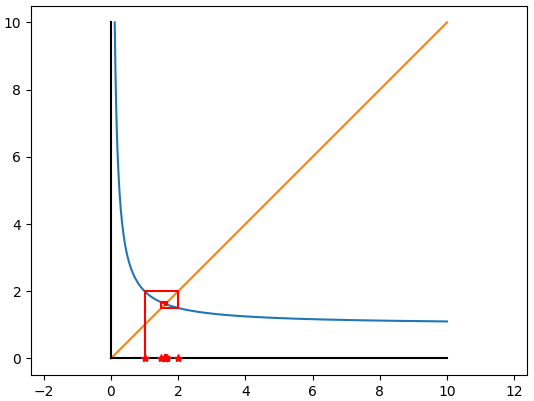
\includegraphics[scale = 0.5]{./img/Figure_8.png}
            \end{subfigure}

            \vspace{\baselineskip}
            
            \begin{subfigure}[b]{0.49\textwidth}
            \centering
            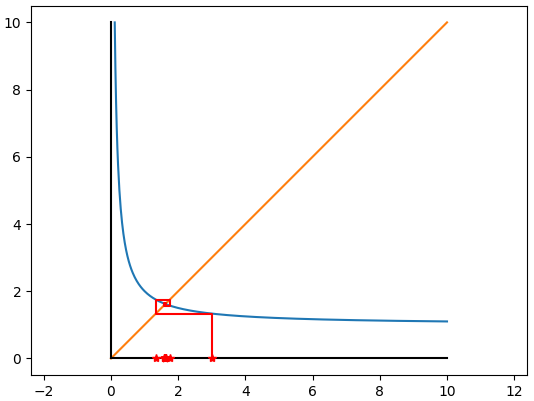
\includegraphics[scale = 0.5]{./img/Figure_9.png}
            \end{subfigure}
            \begin{subfigure}[b]{0.49\textwidth}
            \centering
            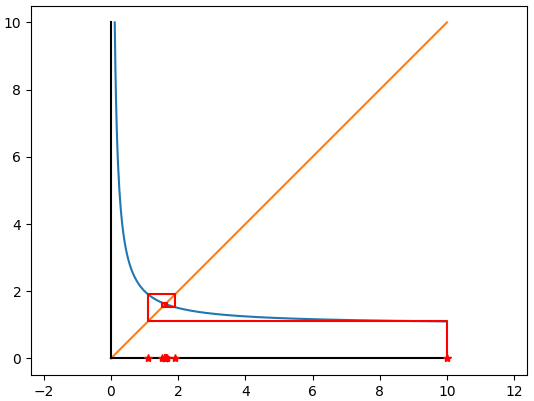
\includegraphics[scale = 0.5]{./img/Figure_10.png}
            \end{subfigure}
        \end{figure}
        \item Si $\alpha = 0$, el único equilibrio del sistema es $l = 1$, y es no hiperbólico porque $|f'(l)| = \frac{1}{l^2} = 1$. Representando gráficamente $f$ y la recta $ y = 2-x$, se observa que $f$ es esctricamente decreciente y $f(x) > 2-x$ para todo $x \in (0,\infty)$, así que $l$ es un equilibrio inestable.
        
        También se verifica $f^2(x) = x$ para todo $x > 0$, así que para $x,y \in (0,1) \cup (1,\infty)$ cualesquiera con $x \neq y$, se tiene que $\{x,y\}$ es una órbita $2$-periódica. En consecuencia, todas las sucesiones de la forma
        \[\begin{cases}
            x_0 \in (0,1)\cup (1,\infty), \\
            x_{n+1} = f(x_n), \qquad n = 0,1,2,\mathellipsis,
        \end{cases}\]
        no convergen, pues no son más que $\{x_0,\frac{1}{x_0},x_0,\frac{1}{x_0},x_0,\mathellipsis\}$.
    \end{enumerate}
\end{solution}

\end{document}